\subsection*{Punto 02}

\textbf{Calcula y muestra el índice Fowlkes Mallows score (FM) usando el conjunto de entrenamiento. Muestra en una gráfica FM como una función de k, y comenta al respecto. Qué valor de k maximiza este criterio?}

En la figura \ref{fig:fowlkes_score} se visualiza el ínidice de Fowlkes Mallows para cada k calculada con el conjunto de entrenamiento. El índice de Fowlkes Mallows sigue una forma semejante a la figura \ref{fig:problema_05_minimum_score}. La diferencia se encuentra en el orden de magnitud de los valores de cada score obtenido. Si se quisiera máximizar el índice de Fowlkes Mallows se usaría k=2. Ya que para este valor se obtiene el valor máximo del índice.

\begin{figure}[H]
    \centering
    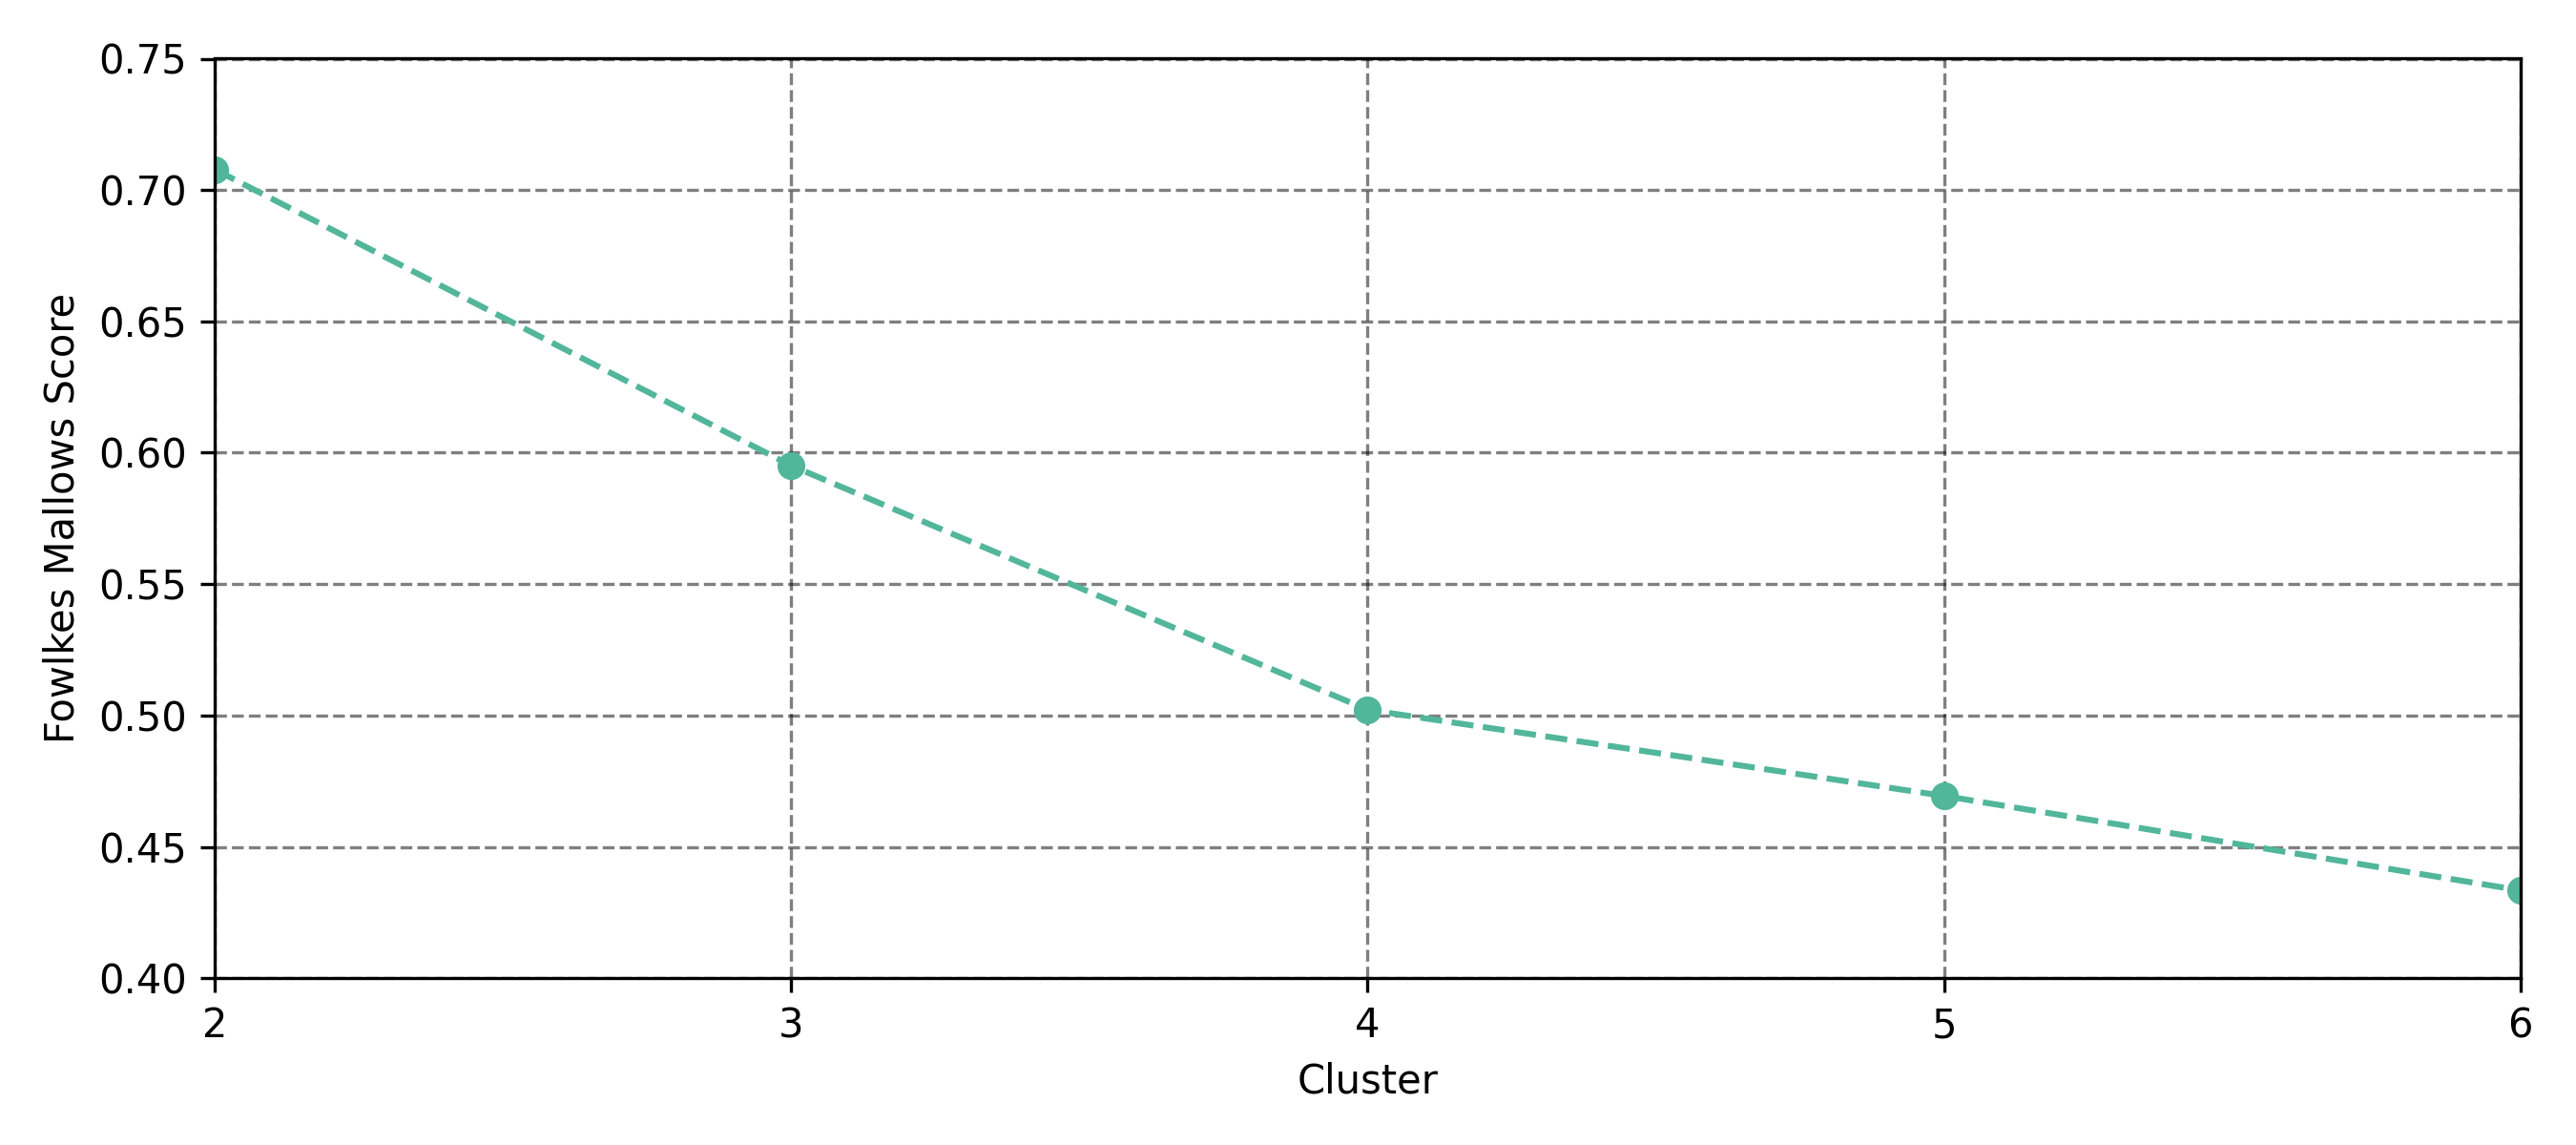
\includegraphics[width=15cm]{Graphics/Problema_05/fowlkes_mallows_score.png}
    \caption{Índice de Fowlkes Mallows obtenido a partir de los resultados usando el conjunto de entrenamiento del dataset \file{creditcard.csv}.}
    \label{fig:fowlkes_score}
\end{figure}